\chapter{Description du capteur} \label{desc_capteur}

Les informations relatives aux sportifs sont acquises par le biais du capteur. Il sera composé d’un assemblage de différents éléments déjà existants dans le commerce. On veillera à minimiser au maximum son poids ainsi que sa taille pour éviter de gêner le sportif durant sa course. Une fois assemblé, il sera placé dans une boîte étanche qui disposera d’un bracelet élastique ce qui permettra à l’athlète de le porter facilement. Enfin il doit également disposer de sa propre source d’énergie sous la forme d’une batterie, celle-ci doit lui conférer une autonomie assez grande pour pouvoir fonctionner durant l’entièreté d’une course.

Trois types de données différentes seront récupérées, la position GPS du coureur (longitude/latitude), son rythme cardiaque en battement par minute ainsi que la cadence de ses pas en pas par minute. Régulièrement le capteur va effectuer les acquisitions nécessaires, puis il va traiter les données et créer un paquet de données. Une fois que le paquet est prêt à être transmis, le capteur utilise son module de transmission LoRa pour les envoyer à la passerelle. 

Le capteur se base sur un système d'exploitation temps réel qui lui permet de définir plusieurs tâches différentes exécutés en parallèle, chacune responsable d'une opération spécifique. La tâche principale sera responsable, à intervalles réguliers, de paquetiser et d'envoyer les données qui auront été acquises durant une période donnée. Une autre tâche sera en charge de la récupération et de l'extraction de la position GPS depuis un message NMEA. Enfin une tâche sera dédiée au comptage du nombre de pas et une autre au comptage du nombre de battement du cœur.

De manière générale, le processus du capteur est illustré par la figure ~\ref{fig:proc_capteur}.

\begin{figure}[htb]
\centering 
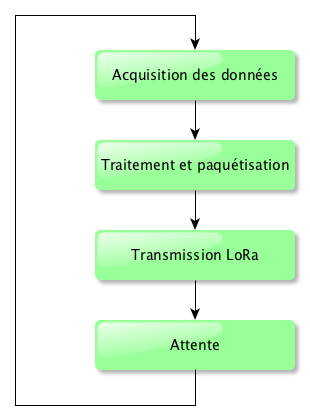
\includegraphics[width=0.4\columnwidth]{../images/capteur_flowchart.png} 
\caption[Processus Capteur]{Processus du capteur}
\label{fig:proc_capteur}
\end{figure}

Le microcontrôleur est la partie centrale du capteur, c’est lui qui exécute le programme d’acquisition des différents paramètres décrit ci-dessus, qui fait le traitement des données pour ensuite les envoyer en utilisant la transmission LoRa. Le cœur du capteur sera donc un module disposant d’un microcontrôleur ainsi que tout ce qui lui ai nécessaire pour fonctionner (oscillateur, mémoire, interfaces…).

Viendront se coupler au microcontrôleur les quatre modules suivants :
\begin{itemize}
\item Un module GPS permettant le positionnement du coureur
\item Un module permettant la mesure du rythme cardiaque
\item Un module accéléromètre qui donnera la possibilité de déterminer la cadence du coureur
\item Un module radio LoRa avec antenne qui se chargera de la communication avec la passerelle\\
\end{itemize}

Le microcontrôleur devra communiquer avec chacun de ses modules d’une manière ou d’une autre afin de pouvoir récupérer les informations et les transmettre. Les modules n’ont pas les mêmes contraintes, il est donc impératif de sélectionner un environnement dans lequel chacun d’eux aura à disposition le canal de communication approprié que ce soit une interface série, un I/O ou un bus SPI par exemple.

Les prochaines sections de ce chapitre décrivent chaque module ainsi que leurs interfaces.

\section{Position GPS}

Un module GPS est responsable de déterminer la position du coureur. Le système GPS se base sur une constellation d’au moins 24 satellites qui sont en orbite moyenne (Altitude de 20'200 km) autour de la Terre. Afin qu’un utilisateur puisse déterminer sa position sur le globe, il est nécessaire qu’il ait la vue sur au moins 4 satellites. A une fréquence très précise, donné par des horloges atomiques, les données de position orbitales ainsi que de temps sont envoyées en direction de la planète, grâce à ses informations le receveur est en mesure de connaître la distance de chacun des satellites en vue et donc de calculer sa position géographique ainsi que de déterminer le temps actuel, c’est ce que l’on appelle le GPS « lock » ou « fix ». \cite{gps_overview}

Cette tâche compliquée est entièrement à la charge du module GPS lui-même, il dispose d’une antenne qui lui permet de recevoir les données envoyées par les satellites, de les analyser et de calculer les informations requises pour les mettre à disposition du microcontrôleur.
La grande majorité des modules GPS transmettent les informations en utilisant une interface série UART sur lequel des messages de type NMEA 0183 sont envoyé vers le récepteur. Ce protocole définit le format de plusieurs messages qui contiennent diverses informations de position, de statuts et de temps. \cite{nmea_0183}

Dans le cadre du projet de Bachelor l’information principale qui sera exploité sera la longitude et latitude du capteur qui permettra de déterminer la position du coureur. D’autres informations intéressantes pourront éventuellement être utilisées comme le temps ou l’altitude.

Le composant peut être directement placé sous l’antenne ou alors il existe également des solutions avec antenne branché par un câble comme montré sur la figure~\ref{fig:antenne_gps}.

\begin{figure}[htb]
\centering 
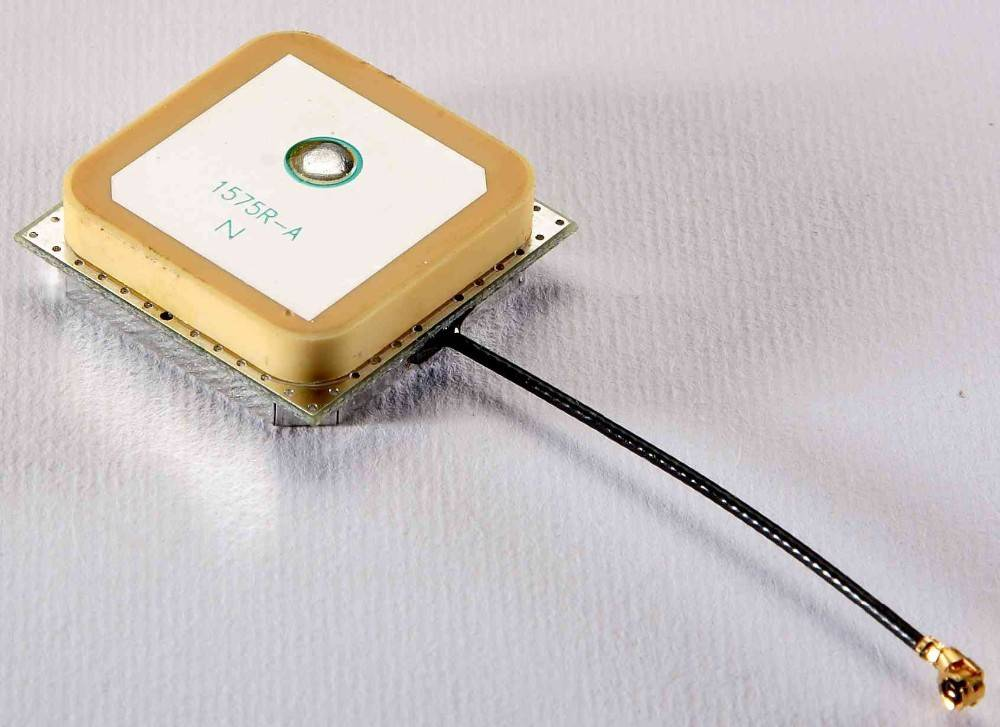
\includegraphics[width=0.5\columnwidth]{../images/active-gps-antenna-large.jpg} 
\caption[Antenne GPS]{Antenne GPS - © SODAQ}
\label{fig:antenne_gps}
\end{figure}

\section{Rythme cardiaque}

Il existe deux moyens principaux de déterminer le rythme cardiaque d’une personne. La première solution consiste à utiliser une ou plusieurs électrodes qui détecteront directement les signaux électriques émit par le cœur, c’est le principe utilisé par les électrocardiogrammes. L’autre solution est basée sur l’utilisation de LEDs placés contre la peau et qui vont émettre de la lumière à une fréquence régulière, la lumière réfléchie par réfraction et qui dépend de la dilatation des vaisseaux sanguins est ensuite détecté par le capteur et permet de déterminer le rythme cardiaque de l’utilisateur. Cette deuxième technique est très utilisée dans les montres GPS utilisés pour le sport car elle a l’avantage de pouvoir être directement intégrée dans le boîtier et ne nécessite que peu de moyen pour être mis en place.

Pour le capteur de ce projet, les deux solutions existent sur le marché, cependant la solution de l’électrocardiogramme semble plus appropriée et pratique car elle permet d’utiliser un cardiofréquencemètre sans fil du commerce et évite ainsi au porteur du capteur de devoir s’accommoder des fils qui sont nécessaire pour le fonctionnement de la solution à base de LED.

Dans les deux cas, l’utilisation par le microcontrôleur est semblable, la sonde sera connectée sur une entrée digitale et elle émettra une impulsion à chaque fois qu’un battement sera détecté. Il suffit donc de compter le nombre d’impulsion et de mesurer le temps pendant lesquels elles ont eu lieu pour pouvoir déterminer la fréquence cardiaque en BPM (Battement par minute).

La formule~\ref{eqn:rythme_card} permet de calculer le rythme cardiaque~$rc$ en battement par minutes (BPM).

\begin{equation}\label{eqn:rythme_card}
rc = \frac{60 * n}{t}
\end{equation}

Avec~$n$ le nombre de battement accumulé pendant un temps~$t$ en secondes.

Les battements du cœur peuvent être détecté grâce à une sangle pectorale munie d’un cardiofréquencemètre. Adafruit propose ce genre de dispositif, il émet une impulsion chaque fois qu'un battement est détecté, un petit module connecté sur une ligne d'entrée du microcontrôleur permet ensuite au logiciel de les compter. Ce type de dispositif est illustré sur la figure~\ref{fig:cardiofreq}. Du fait de la gêne occasionnée par une électrode cette solution sera privilégiée.

\begin{figure}[htb]
\centering 
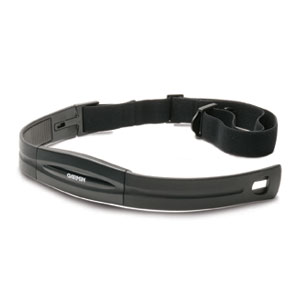
\includegraphics[width=0.35\columnwidth]{../images/garmin-heart-rate.jpg} 
\caption[Sangle Pectorale]{Sangle pectorale - © Garmin}
\label{fig:cardiofreq}
\end{figure}

\section{Cadence de pas}

Le nombre de pas effectué pendant un certain temps, c’est-à-dire la cadence, est une information intéressante pour les coureurs. Tout un tas de facteur peuvent l’influencer, comme le poids, la taille ou la longueur des jambes. Les coureurs amateurs se trouvent en général dans la tranche de 160 à 170 pas par minute alors que des coureurs d’élites à 180 ou même 200 pas par minute lorsqu’ils sont au maximum de leur vitesse. La cadence permet de juger de la bonne posture d’un coureur, plus les pas seront cours et plus la cadence sera élevée. 

De manière générale, en course à pied la préférence est portée sur les petits pas, d’une part car c’est uniquement lorsque le coureur touche le sol qu’il peut donner une impulsion vers l’avant, ce qui lui permet d’aller plus vite, et d’autre part car le fait de faire des grands pas augmente le risque de blessure, le pied a tendance à taper plus fort sur le sol. Une cadence plus élevée permet d’améliorer la position où le pied touche le sol, idéalement cela devrait être directement en dessous du centre de gravité ou lieu de plus en avant.

Afin de déterminer la cadence de pas, un module accéléromètre est utilisé. Ce type de composant permet de mesurer l’accélération linéaire soit en \SI{}{\m\per\square\s} ou en g sur un ou plusieurs axes, en général les axes X, Y et Z. Plusieurs interfaces de communication existent pour ce type de composant, analogique ou les niveaux sont transmis à travers des valeurs de voltage, digitale avec un bus I2C ou SPI ou alors grâce à une modulation de largeur d’impulsion (PWM). Pour ce projet une communication digitale de type I2C ou SPI sera privilégiée afin de simplifier la récupération des données de l’accéléromètre.

Beaucoup d’application qui utilise ce composant existe, il permet par exemple de détecter l’orientation d’un téléphone portable (paysage ou portrait) ou de savoir si un objet est en mouvement. C’est également l’élément central des podomètres, qui permettent de compter le nombre de pas effectué, gadget qui est très à la mode en ce moment. C’est justement cette application qui sera utilisée dans le cadre du projet, il faudra compter le nombre de pas effectué par le coureur en un certain temps pour déterminer sa cadence.

Afin de détecter quand la personne fera un pas, il est nécessaire de pouvoir détecter un pic d’accélération dans une ou plusieurs directions. Il faudra déterminer un pallier au-dessus duquel on considérera que l’intensité de l’accélération est suffisamment élevée pour la considérer comme un pas. Pour se faire il faudra que le programme lise les informations des différents axes de l’accéléromètre régulièrement et qu’il les analyse, ceci lui permettra de garder un compte du nombre de pas. Il faudra également mesurer le temps durant lequel les pas ont été comptés pour pouvoir calculer la cadence à un certain moment. 

Au lieu que le programme fasse lui-même les acquisitions, certains accéléromètres peuvent être configuré pour déclencher une interruption lorsqu’un certain seuil est dépassé, cette méthode dépend entièrement du composant utilisé cependant dans la mesure du possible elle sera privilégiée car elle facilite le traitement de cette activité et évite une surcharge des opérations requises par le logiciel.

De manière similaire au rythme cardiaque, la cadence de pas~$cp$ en pas par minute pourra être calculée avec la formule~\ref{eqn:cadence_pas}.

\begin{equation}\label{eqn:cadence_pas}
cp = \frac{60 * n}{t}
\end{equation}

Avec~$n$ le nombre de pas accumulé pendant un temps~$t$ en secondes.

\section{Radio LoRa}

La partie radio LoRa, c’est-à-dire la transformation des données en ondes radio est à la charge d’un composant spécifique. Il existe deux principaux types de composant, le premier intègre uniquement la couche physique LoRa, le deuxième en plus de cette couche propose également la couche protocolaire LoRaWAN. Comme expliqué dans ce document, dans le cadre du projet seule la couche radio LoRa sera employée, les composants intégrant la couche LoRaWAN offre toujours la possibilité d’utiliser uniquement la couche radio, il sera donc possible d’utiliser l’un ou l’autre de ses types de composant pour le projet.

La majorité des modules radio LoRa existant sur le marché proposent en règle générale uniquement la gestion de la couche physique, cette partie étant la propriété de la société Semtech, les composants embarqués sont toujours les mêmes, soit le composant SX1272 ou le SX1276. Ils communiquent les deux avec le microcontrôleur au moyen d’un bus SPI.

\section{Matériel}

Ce chapitre décrit une série de composants qui pourront être utilisé dans l’assemblage final du capteur. La sélection des composants exacts utilisés pour le travail de Bachelor se fera au début de la phase de réalisation.

Il est possible que certains de ses modules soit directement intégré au module microcontrôleur, il existe sur le marché des solutions qui en plus du microcontrôleur dispose également du module radio LoRa ou d’un GPS par exemple. Ce genre de configuration permet un gain de place et de temps car les composants sont montés sur un seul et même PCB.

\subsection{Adafruit Feather}

La société Adafruit a développée toute une suite de produits différents dont les Feather et les Featherwing. L’objectif des Feather est de proposer des cartes électroniques légères, de petite taille, pouvant être alimenté par batterie et proposant tout un panel de configuration et périphérique différents. Les Featherwing quant à elle sont des cartes d’extension qui vienne se ficher par-dessus un Feather et qui permette d’ajouter les fonctions additionnelles désirées.

Dans cette gamme il existe plusieurs modules pouvant être utilisé pour le projet, le plus approprié est le Feather M0 with RFM95 LoRa Radio, le module intègre directement un microcontrôleur ainsi qu’un module radio LoRa couche physique. Il est également possible d’y brancher une batterie lithium-ion.

\begin{figure}[htb]
\centering 
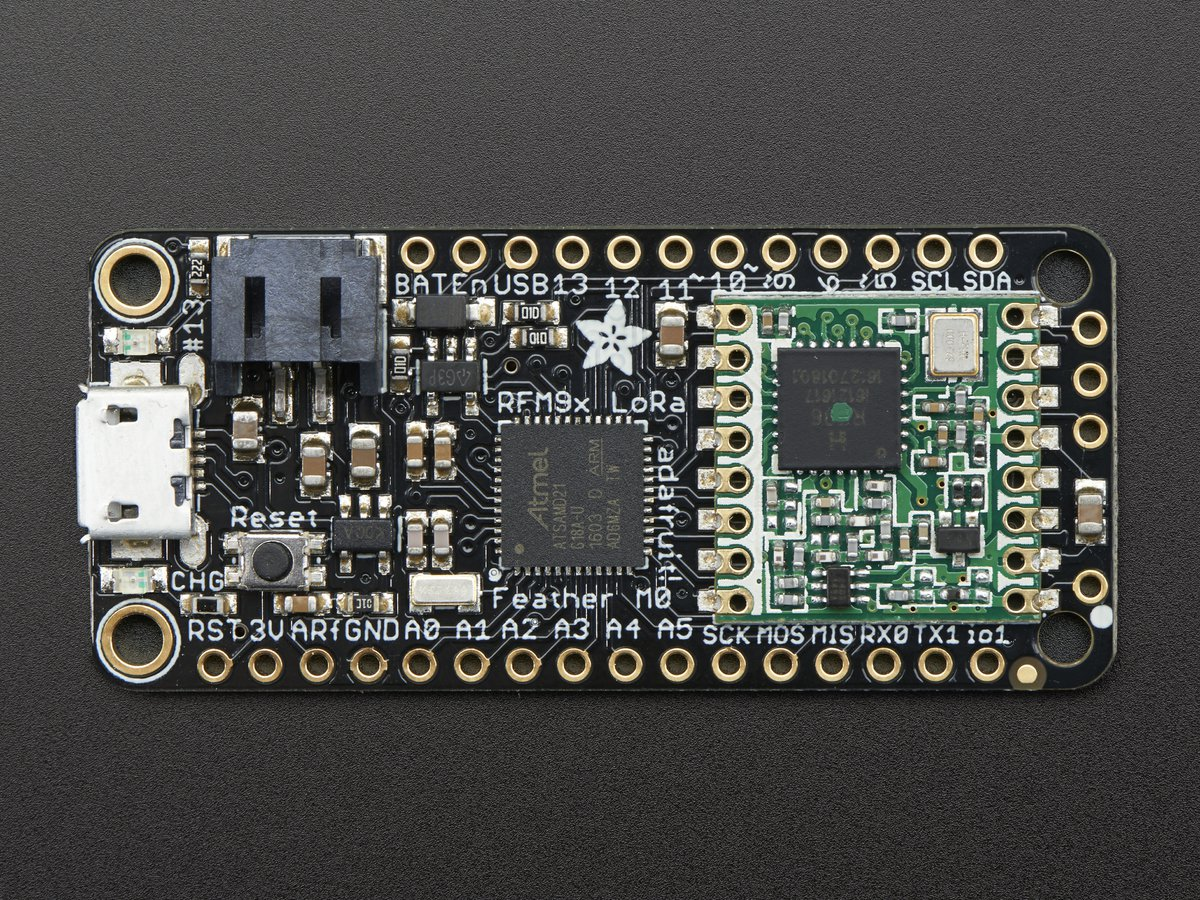
\includegraphics[width=0.4\columnwidth]{../images/adafruit-feather-m0-lora.jpg} 
\caption[Adafruit Feather]{Feather M0 with RFM95 LoRa Radio - © Adafruit}
\label{fig:ada_feather}
\end{figure}

Les caractéristiques du microcontrôleur sont résumées dans la table~\ref{tab:ada_feather_cara}.

\begin{table}[htb]
\caption[Adafruit Feather Caractéristiques]{Caractéristiques de la carte Adafruit Feather M0}
\label{tab:ada_feather_cara}
\centering
\begin{tabular}{ l | l }
\toprule
Dimensions & 51mm x 23mm x 8mm \\
\midrule
Microcontrôleur & ATSAMD21G18 – ARM Cortex M0 \\
\midrule
Oscillateur & 48 Mhz \\
\midrule
Flash & 256 kB \\
\midrule
RAM & 32 kB \\
\midrule
LoRa & Semtech SX1272 \\
\midrule
Prix & 34.50 CHF\\
\bottomrule 
\end{tabular}
\end{table}

Pour la gestion du GPS, on pourra s’appuyer sur le Adafruit Ultimate GPS Featherwing illustré par la figure~\ref{fig:ada_featherwing_gps}, qui propose un module pouvant se fixer sur le module de base avec un composant de gestion de la position. Une connexion série UART sera utilisée pour récupérer les messages NMEA et ainsi pouvoir en extraire la position du module.

\begin{figure}[htb]
\centering 
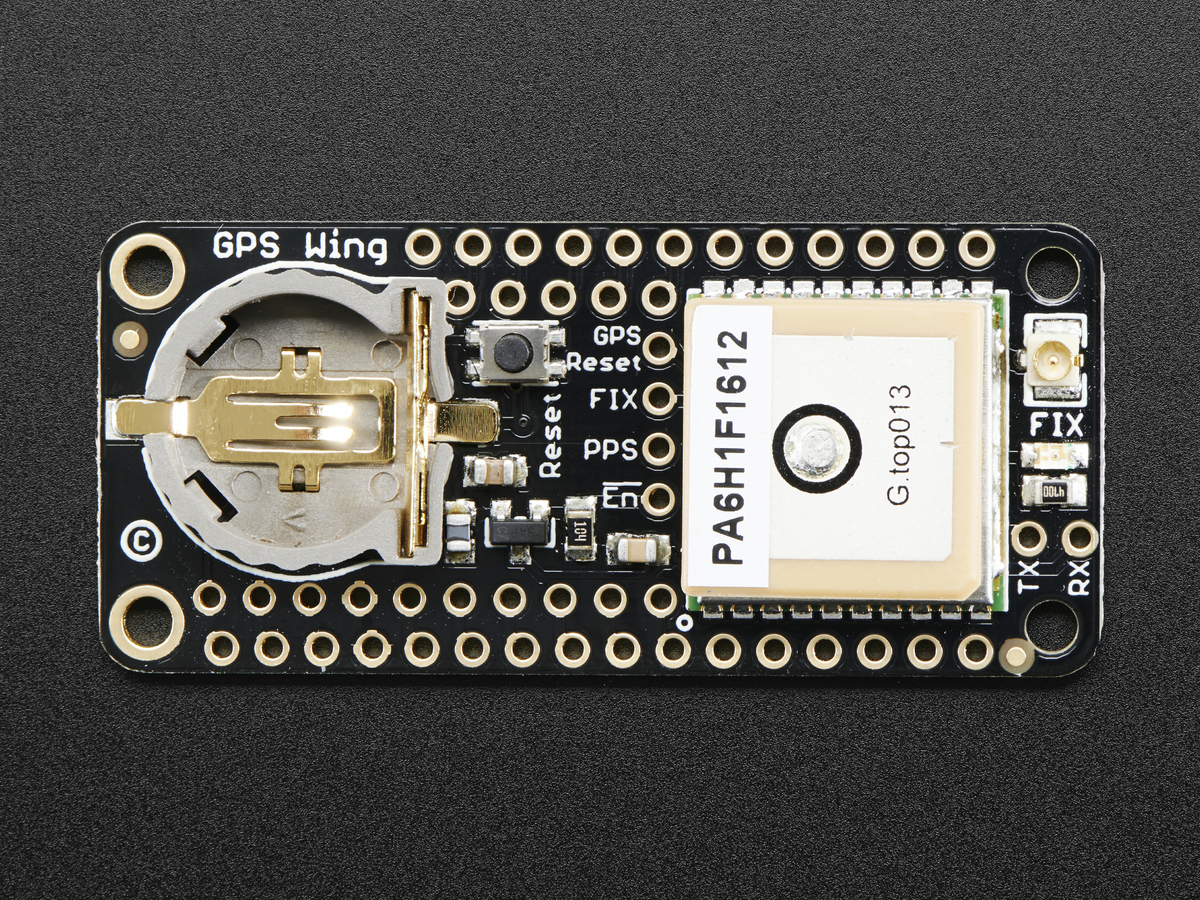
\includegraphics[width=0.4\columnwidth]{../images/adafruit-featherwing-ultimate-gps.jpg} 
\caption[Adafruit Featherwing GPS]{Adafruit Ultimate GPS Featherwing - © Adafruit}
\label{fig:ada_featherwing_gps}
\end{figure}

En ce qui concerne la partie logiciel, quelques systèmes d’exploitation temps réel existe pour ce type de processeur ARM. Pour ce développement l’utilisation de Zephyr sera privilégiée car il propose toutes les fonctionnalités standard que l’on pourrait attendre de ce type de système d’exploitation, une configuration de la carte Adafruit Feather existe déjà et sa communauté est très active.

La table~\ref{tab:ada_feather_liste} propose une liste de l'ensemble des modules nécessaire pour l'assemblage du capteur.

\begin{table}[htb]
\caption[Adafruit Feather List]{Liste de module pour Adafruit Feather}
\label{tab:ada_feather_liste}
\centering
\begin{tabular}{lcc}
\toprule
Module & Prix & Num. produit \\ 
\midrule
Adafruit Feather M0 & 34.05 CHF & ADAFRUIT-3178 \\
Adafruit Heart Rate Start Pack & 65 CHF & ADAFRUIT-1077 \\
Adafruit Triple-Axis Accelerometer & 8 CHF & ADAFRUIT-2019 \\
Adafruit Ultimate GPS FeatherWing & 40 CHF & ADAFRUIT-3133 \\
\midrule
Prix Total & 147.50 CHF &  \\
\bottomrule 
\end{tabular}
\end{table}

\subsection{SODAQ One}

La société Néerlandaise SODAQ propose un module nommé SODAQ One qui contient un microcontrôleur, le même que sur la solution Adafruit, un module LoRa, un accéléromètre ainsi qu’un module GPS sur le même PCB. Cette solution a l’avantage de contenir directement pratiquement tous les modules nécessaires au projet, reste la sonde de rythme cardiaque à intégrer. 

Il est possible d’alimenter le SODAQ One avec une batterie lithium-ion, un petit panneau solaire est également proposé. Autre avantage de taille de cette carte est le fait qu’elle embarque le module LoRa de Microchip RN2483 qui propose la gestion de la couche physique LoRa ainsi que de la couche protocolaire LoRaWAN. Une interface série de type UART en utilisé pour envoyer des commandes à la puce de gestion du LoRa, elle permet aussi l’utilisation de la couche radio uniquement ou alors en consort avec la couche protocolaire. La figure~\ref{fig:sodaq_one} montre l'allure du module SODAQ One.

\begin{figure}[htb]
\centering 
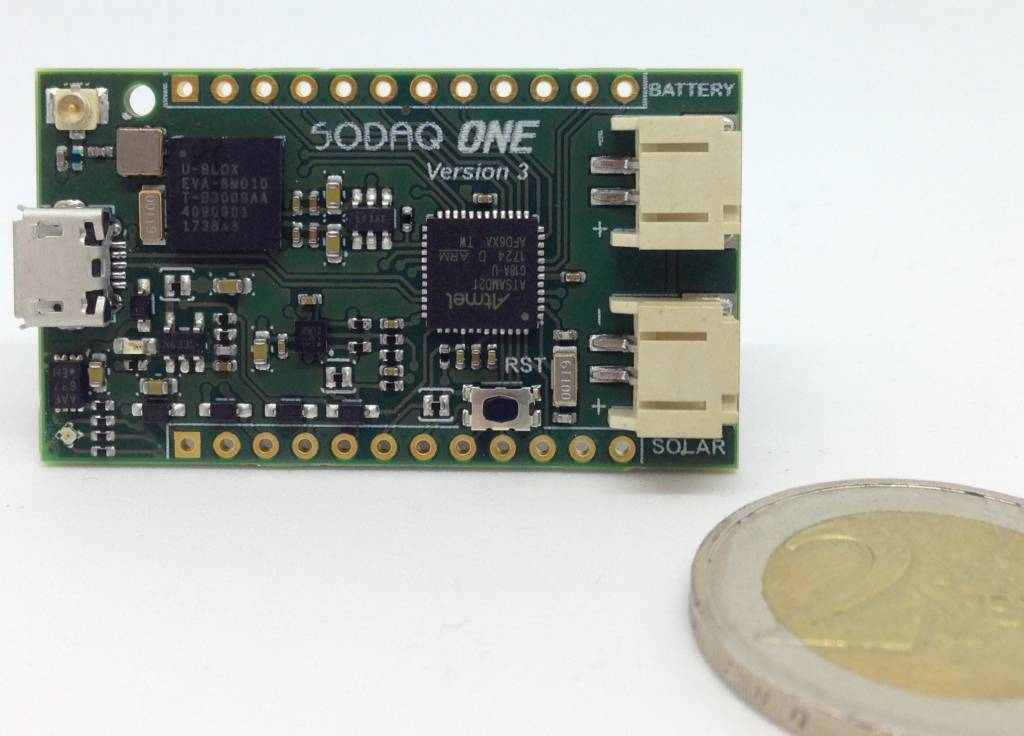
\includegraphics[width=0.4\columnwidth]{../images/sodaq-one-eu-rn2483-v3.jpg} 
\caption[SODAQ One]{SODAQ One v3 - © SODAQ}
\label{fig:sodaq_one}
\end{figure}

Les caractéristiques du microcontrôleur sont résumées dans la table~\ref{tab:sodaq_one_cara}.

\begin{table}[htb]
\caption[SODAQ One Caractéristiques]{Caractéristiques de la carte SODAQ One v3}
\label{tab:sodaq_one_cara}
\centering
\begin{tabular}{ l | l }
\toprule
Dimensions & 45mm x 25mm \\
\midrule
Microcontrôleur & ATSAMD21G18 – ARM Cortex M0 \\
\midrule
Oscillateur & 48 Mhz \\
\midrule
Flash & 256 kB \\
\midrule
RAM & 32 kB \\
\midrule
LoRa & Microchip RN2483 \\
\midrule
GPS & uBlox EVA 8M \\
\midrule
Accéléromètre & STMicroelectronics LSM303AGR \\
\midrule
Prix & 114 CHF\\
\bottomrule 
\end{tabular}
\end{table}

C’est cette solution qui requiert le moins de travail de modification ou d’ajout pour pouvoir couvrir tous les aspects requis par le projet. Sa petite taille la rend également idéale pour l’utilisation pour ce travail de Bachelor.

Puisque le microcontrôleur utilisé par ce capteur est le même que la solution Adafruit, en termes de logiciel le même système d’exploitation temps réel sera utilisé, c’est-à-dire Zephyr.

La table~\ref{tab:sodaq_one_liste} propose une liste de l'ensemble des modules nécessaire pour l'assemblage du capteur.

\begin{table}[htb]
\caption[SODAQ One List]{Liste de module pour SODAQ One}
\label{tab:sodaq_one_liste}
\centering
\begin{tabular}{lcc}
\toprule
Module & Prix & Num. produit \\ 
\midrule
SODAQ One v3 & 114 CHF & ONE-EU-RN2483-V3 \\
Adafruit Heart Rate Start Pack & 65 CHF & ADAFRUIT-1077 \\
\midrule
Prix Total & 179 CHF &  \\
\bottomrule 
\end{tabular}
\end{table}

\subsection{Multiconnect mDot}

La société Multitech propose plusieurs modules de taille et de spécifications différentes, l’un d’eux est le mDot, un module de petite taille qui incorpore un microcontrôleur ainsi qu’un module radio LoRa. Il n’embarque pas d’autre module utile au projet cependant son avantage réside dans le fait qu’il donne la possibilité d’utiliser le système d’exploitation temps réel mBed qui offre toutes les fonctionnalités généralement proposées pour la gestion du temps réel comme la création de tâches, de sémaphores ou d’évènements. Cet environnement de développement est également composé d’une couche LoRaWAN logiciel permettant l’envoie de donnée à une passerelle.

\begin{figure}[htb]
\centering 
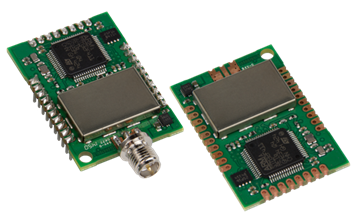
\includegraphics[width=0.5\columnwidth]{../images/Multitech-mDot.png} 
\caption[Multitech mDot]{Multitech mDot - © Multitech}
\label{fig:multitech_mdot}
\end{figure}

Les caractéristiques du microcontrôleur sont résumées dans la table~\ref{tab:multitech_mdot_cara}.

\begin{table}[htb]
\caption[Multitech mDot Caractéristiques]{Caractéristiques de la carte Multitech mDot}
\label{tab:multitech_mdot_cara}
\centering
\begin{tabular}{ l | l }
\toprule
Dimensions & 37.3mm x 25.5mm \\
\midrule
Microcontrôleur & STM32F411RET – ARM Cortex M4 \\
\midrule
Oscillateur & 96 Mhz \\
\midrule
Flash & 512 kB \\
\midrule
RAM & 128 kB \\
\midrule
LoRa & Semtech SX1272 \\
\midrule
Prix & 53 CHF\\
\bottomrule 
\end{tabular}
\end{table}

L’avantage principal de cette solution est que le module vient accompagner par une suite logicielle complète et bien documenté permettant le développement d’une application temps réel. Par contre il nécessite la mise en place d’une carte supplémentaire afin de pouvoir y placer tous les autres composants nécessaires, c’est-à-dire le module GPS, l’accéléromètre et la sonde de rythme cardiaque, ce qui rajoute une quantité de travaille non négligeable ainsi que des risques accrus de rencontrer des problèmes.

La table~\ref{tab:mdot_liste} propose une liste de l'ensemble des modules nécessaire pour l'assemblage du capteur.

\begin{table}[htb]
\caption[Multitech mDot List]{Liste de module pour Multitech mDot}
\label{tab:mdot_liste}
\centering
\begin{tabular}{lcc}
\toprule
Module & Prix & Num. produit \\ 
\midrule
Adafruit Feather M0 & 34.05 CHF & MTDOT-868-X1-SMA \\
Adafruit Heart Rate Start Pack & 65 CHF & ADAFRUIT-1077 \\
Adafruit Triple-Axis Accelerometer & 8 CHF & ADAFRUIT-2019 \\
Adafruit Ultimate GPS Breakout & 40 CHF & ADAFRUIT-746 \\
\midrule
Prix Total & 166 CHF &  \\
\bottomrule 
\end{tabular}
\end{table}

\subsection{Comparatif des différents modules}

Cette section vise à comparer les modules entre eux pour pouvoir évaluer les avantages et inconvénients de chacun d’entre eux, ce qui facilitera la sélection du module qui sera utilisé durant le travail de Bachelor.

\begin{table}[htb]
\caption[Comparatif Microcontroleur]{Comparatif des caractéristiques des modules}
\label{tab:comparatif_micro}
\centering
\begin{tabular}{lcccccccc}
\toprule
Module & Prix & Microcontrôleur & Fréquence & Flash & RAM  \\ 
\midrule
Adafruit Feather M0	& 34.50 CHF	& ATSAMD21G18 & 48 Mhz & 256 kB & 32 kB & \\
SODAQ One	& 114 CHF & ATSAMD21G18 & 48 Mhz & 256 kB & 32 kB \\
Multiconnect mDot & 53 CHF & STM32F411RET & 96 Mhz & 512 kB & 128 kB \\
\bottomrule 
\end{tabular}
\end{table}

\begin{table}[htb]
\caption[Comparatif Module]{Comparatif des différents modules nécessaire}
\label{tab:comparatif_modules}
\centering
\begin{tabular}{lcccccccc}
\toprule
Module & LoRa & LoRaWAN & GPS & Accéléromètre & Rythme Cardiaque \\ 
\midrule
Adafruit Feather M0	& SX1272	& Librairie tierce & x & x & x  \\
SODAQ One	& RN2483	& RN2483 & \checkmark & \checkmark & x \\
Multiconnect mDot & SX1272 & Librarie mDot & x & x & x \\
\bottomrule 
\end{tabular}
\end{table}

Si l’on analyse le contenu des tableaux, on remarque que le module SODAQ One se détache des deux autres solutions. Il propose déjà deux des trois fonctionnalités demandées par le projet, le GPS et l’accéléromètre, reste le rythme cardiaque à intégrer qui ne requiert à priori qu’une simple ligne I/O. De plus ce module propose une solution LoRa intéressante grâce à la puce RN2483 produite par Microchip commandé par un lien série UART, ce qui rend la gestion de la communication et l’envoie de donnée plus simple.

Le module mDot de la société Multitech représente une solution intermédiaire avec plus de flexibilité dans le choix des composants utilisé, de base elle ne propose aucun des modules requis pour le projet. Son avantage principal réside dans le fait que le module est fourni avec une suite logicielle complète comprenant un système d’exploitation temps réel, mBed, ainsi que plusieurs librairies pour la gestion des communications. Pour cette solution un travail plus substantiel sera nécessaire pour ajouter les modules nécessaires au projet.

Finalement la solution Adafruit Feather représente une somme de travail conséquente, il faudra prévoir l’ajout d’un accéléromètre ainsi que d’une sonde pour le rythme cardiaque. L’avantage principal de cette solution est son prix bas ainsi que la possibilité de ficher le module GPS par-dessus le module de base ce qui permet un gain en termes de place ce qui est intéressant dans une optique de minimiser la taille du capteur.
